% !TEX root = ..\main.tex
\chapter{Experiments}\label{ch:Experiments}

\section{Experiment 1: Comparison}\label{sec:Exp1}
The goal of this experiment is to provide validation of the implementation in the PoC. This is done with the results of the paper \textit{"A Comprehensive Study of Bloated Dependencies in the Maven Ecosystem"} by Soto-Valero et al. \cite{soto2020comprehensive}. In this work, a byte-code analysis is performed on Maven Artifacts to detect which of the dependencies of this artifacts are \textit{bloated}, which we refer to as \textit{unused}. Although the PoC created in this thesis does not perform exactly the same kind of analysis, we consider that a dependency is \textit{unused} if no usage is detected by any of the metrics in the model.

\subsection{Experimental set up}
Soto-Valero et al. perform a qualitative analysis, in which they analyze 31 libraries available as Maven artifacts. If unused dependencies are found during the analysis, a \textit{Pull Request} is made to the \textit{GitHub} repository of the artifact in which the unused dependencies are deleted from the \textit{pom} file.

With the information in the paper, we collect the \textit{GroupId} and \textit{ArtifactId} of the 31 artifacts. Out of the 31, 2 could not be found in the \textit{Maven Repository Central}. For the other 29, the \textit{version} to use in the experiment is determined by finding the last version released before the experiment by Soto-Valero et al. was conducted - November of 2019.

Of the 29 artifacts, 13 could not be used with the PoC, because either the artifact itself or some dependency could not be downloaded from \textit{Maven Central}, leaving a set of 16 libraries to analyse and compare the results with the results obtained by Soto-Valero et al. The table containing the identifiers of the artifacts used in this experiment can be found in Table \ref{table:comparison-artifacts}.

\begin{table}[ht]
    \begin{center}
    \begin{tabular}{|l|l|l|}
    \hline
    Group Id              & Artifact Id                     & Version       \\
    \hline
    org.mybatis           &	mybatis	                        & 3.5.3         \\
    org.apache.flink      & flink-core                      & 1.9.1         \\
    com.puppycrawl.tools  & checkstyle                      & 8.27          \\
    com.google.auto       & auto-common                     & 0.10          \\
    edu.stanford.nlp      & stanford-corenlp                & 3.9.2         \\
    com.squareup.moshi    & moshi-kotlin                    & 1.9.2         \\
    org.neo4j             & neo4j-collections               & 3.5.13        \\
    org.asynchttpclient   & async-http-client               & 2.10.4        \\
    org.alluxio           & alluxio-core-transport          & 2.1.0         \\
    com.github.javaparser & javaparser-symbol-solver-logic  & 3.15.5        \\
    io.undertow           & undertow-benchmarks             & 2.0.27.Final  \\
    org.teavm             & teavm-core                      & 0.6.1         \\
    com.github.jknack     & handlebars-markdown             & 4.1.2         \\
    ma.glasnost.orika     & orika-eclipse-tools             & 1.5.4         \\
    fr.inria.gforge.spoon & spoon-core                      & 8.0.0         \\
    org.jacop             & jacop                           & 4.7.0         \\
    \hline
    \end{tabular}
    \end{center}
    \caption{Identifiers of the Maven artifacts used for comparison}
    \label{table:comparison-artifacts}
\end{table}

The first idea was to create a request that computed the comparison automatically. However, finding the reason why the results were not exactly the same, in most of the cases needed manual checking and research. That is why, the analysis of the libraries in Table \ref{table:comparison-artifacts} have been executed one by one, and the comparison has been done manually.

\subsection{Results}

The results obtained from the comparison with the data from the research by Soto-Valero et al. \cite{soto2020comprehensive} is done in two parts: if all the libraries found as unused in the paper are also found as unused by the tool, and if all the other libraries are found as used. For the first part, there are several cases:

\begin{itemize}
  \item \textbf{Correct:} All the dependencies detected as unused in the paper, are also detected as unused by the PoC.
  \item \textbf{Testing:} At least one of the unused dependencies is a testing depenedency, and therefore it is not detected by the PoC.
  \item \textbf{Parent:} At least one of the unused dependencies is from a parent module, and it does not appear in the tree of the artifact.
  \item \textbf{Used:} At least one of the unused dependencies is found as used by the PoC.
\end{itemize}

The cases that can happen for the rest of the libraries, the ones that are found as used by Soto-Valero et al. are listed below:

\begin{itemize}
  \item \textbf{Correct:} All the used dependencies according to the paper, are also used according to the tool.
  \item \textbf{Shadowed:} At least one dependency is detected as unused because it is shadowed within the jar file of the client library in the building process.
  \item \textbf{Testing:} At least one dependency is found as unused since it is only used for testing, but not marked with scope \textit{testing}.
  \item \textbf{Unused:} At least one dependency found as used by the paper, is unused in the analysis of the tool.
\end{itemize}

In Table \ref{table:comparison-results}, there are the results for each one of the client libraries used in the experiments.

\begin{table}[ht]
\begin{center}
\begin{tabular}{|l|l|l|}
\hline
\textbf{Library} & \textbf{Unused in paper} & \textbf{Used in paper} \\ \hline
org.mybatis:mybatis:3.5.3                                   & Testing       & Shadowed        \\ \hline
org.apache.flink:flink-core:1.9.1                           & Testing       & Unused          \\ \hline
com.puppycrawl.tools:checkstyle:8.27                        & Testing       & Correct         \\ \hline
com.google.auto:auto-common:0.10                            & Testing       & Unused          \\ \hline
edu.stanford.nlp:stanford-corenlp:3.9.2                     & Correct       & Unused          \\ \hline
com.squareup.moshi:moshi-kotlin:1.9.2                       & Correct       & Correct         \\ \hline
org.neo4j:neo4j-collections:3.5.13                          & Correct       & Unused          \\ \hline
org.asynchttpclient:async-http-client:2.10.4                & Used          & Shadowed        \\ \hline
org.alluxio:alluxio-core-transport:2.1.0                    & Correct       & Unused          \\ \hline
com.github.javaparser:javaparser-symbol-solver-logic:3.15.5 & Correct       & Correct         \\ \hline
io.undertow:undertow-benchmarks:2.0.27.Final                & Parent        & Correct         \\ \hline
org.teavm:teavm-core:0.6.1                                  & Parent        & Correct         \\ \hline
com.github.jknack:handlebars-markdown:4.1.2                 & Correct       & Unused          \\ \hline
ma.glasnost.orika:orika-eclipse-tools:1.5.4                 & Testing, Used & Correct         \\ \hline
fr.inria.gforge.spoon:spoon-core:8.0.0                      & Used          & Correct         \\ \hline
org.jacop:jacop:4.7.0                                       & Correct       & Testing, Unused \\ \hline
\end{tabular}
\end{center}
\caption{Results of the comparison with Soto-Valero et al. \cite{soto2020comprehensive}}
\label{table:comparison-results}
\end{table}

\subsection{Discussion}
To evaluate the results of this experiment, we will discuss the meaning of the different cases as for detecting unused dependencies. There are 9 cases in which the unused dependencies were not correctly detected. Out of these 9, 4 can completely be fixed, if the tool could also analyze the tests defined in the client library. This could be fixed by doing source-code analysis including the testing, instead of bytecode analysis. In addition, the 2 cases in which the dependencies \todo{check why the parent dependencies are not included}. Finally, there are 3 cases in which there are at least was one dependency which according to the paper should be unused, and it was detected used by the PoC. Therefore, the PoC implementation is overestimating in certain measure the usage of the dependencies.

Next, we take a look at the detection of used dependencies. There are 9 cases in which at least one of the dependencies which were supposed to be used, have no usage detected. Two of these cases, are due to the dependencies being shadowed within the jar of the client library during the build process. Also, one case includes a dependency used for testing. Both these scenarios, could be fixed by doing source-code analysis, since the dependencies would not be shadowed yet. Finally, the other 7 cases include dependencies detected as unused, which according to the paper by Soto-Valero et al. \cite{soto2020comprehensive}. This means that there are still some types of connections which are not detected by the tool (e.g., reflection constructs). Also, we researched the server libraries of these cases, and it includes a case in which the dependency is related to the compilation of the project. Another case involves a client library in which the part that uses the dependency is not shipped with Maven, and therefore it cannot be detected in the jar file. Finally, there are some dependencies which are empty - have no classes. A next step could be to investigate what are these libraries used for, and how to detect it.

\section{Experiment 2: Significance of the coupling metrics}

The goal of this experiment is to validate if the coupling metrics designed in the model, namely \texttt{MIC}, \texttt{AC}, \texttt{TMIC}, and \texttt{TAC}, are a good indicator of the usage of the dependencies by the clients. As a partial validation of the significance of the metrics, we compare it with the results gathered from the usage metrics. We want to know how often it happens, that a dependency is used, either by using classes or methods, and it is detected as uncoupled by the coupling metrics. This way, we know if there are many cases in which a dependency that is only used with a type of connection other than method invocation or field declaration.

\unsure{I'm not sure if this is the right place for the explanation of the failed data recolection, or if it is too long}

The original idea was to measure real-world data about how the clients update the dependencies and their impact on the code. We could then have seen the correlation of this impact with the degree of dependency measured with the coupling metrics. Different approaches were taken to obtain real-world data.

First, we tried to find in GitHub commits in which there had been an update of a dependency. However, the search engine in GitHub does not allow to filter the results by the language of the commit. Therefore, most of the results obtained were not useful. Also, most of the updates are only patches, which require only a bump in the version number of the declared dependency.

Based on these findings, the second approach we took was to look for updates that contained breaking changes. To find the libraries that had these type of changes, and in which versions, we used the \textit{Maven Dependency Dataset} \cite{Raemaekers2013}. Raemaekers et al. used this dataset to analyze the use of semantic versioning and the possible impact of breaking changes \cite{Raemaekers2017}. It is possible to query this dataset to obtain libraries with breaking changes, with version numbers and other libraries that depended on these. However, we need to find the commit of the client library in which the update containing a breaking change was made, and it is not always possible. We considered some of the requirements to be able to analyze a dependency with the PoC. For instance, we need all the dependencies of the client library available in Maven, and testing dependencies cannot be used since they are not analyzed by the tool. Considering all these requirements, it was not possible to obtain enough data for the experiment from the \textit{Maven Dependency Dataset} on time, since all these checks had to be done manually.

Next, we contacted the first author of the paper \textit{"Why and How Java Developers Break APIs"} \cite{Brito2018}, which mines GitHub repositories to find possible breaking changes in APIs, to obtain the dataset of breaking changes created based on their findings. Brito, the author, shared the dataset with us. The dataset includes 24 commits containing breaking changes, which correspond to 19 different libraries. Out of the 25 commits, 12 are from libraries managed by Gradle instead of Maven and cannot be used with the PoC. Besides, we could not find 4 of the commits in GitHub, and 2 others correspond to testing libraries, which are out of the scope of the analysis performed by the PoC. Therefore, there were only 6 breaking changes left, for which 3 the Maven artifact that these belong to had no dependants for which to do the analysis. The last 3 have only one dependant, and therefore is not possible to compare the impact of the breaking changes.

Finally, we tried to manually search for deprecated libraries and other libraries that used them — however, similar problems where encountered. Finding commits which replaced a deprecated dependency and the client library and all the dependencies are available in \textit{Maven Central Repository}, is a manual task that, after multiple hours of work, gave no results.


\subsection{Experimental set up}
To run this experiment, we prepared a new request in the API of the PoC. The request has to contain a path to a txt file (tab delimited). The file has to contain three columns (with headers): Group Id, Artifact Id, and version. For each one of the rows, the analysis of the dependencies is performed. The result of each of the analysis is processed, summarizing all the analysis with the following information:

\begin{itemize}
  \item \textbf{Total number of dependencies:} Number of dependencies of all the analyzed client libraries, including both, direct and indirect.
  \item \textbf{Times coupling metrics were not enough:} Number of dependencies for which all the coupling metrics had value zero, but there where methods and classes found reachable by the usage metrics.
  \item \textbf{Times MIC/TMIC were not enough:} Number of times in which there was usage found, but MIC (or TMIC in the case of transitive dependencies) had value zero.
  \item \textbf{Times AC/TAC were not enough:} Number of times in which there was usage found, but MIC (or TMIC in the case of transitive dependencies) had value zero.
  \item \textbf{List server libraries coupling metrics not enough:} The list of \textit{GroupId}, \textit{ArtifactId}, and \textit{version} of the server libraries for which all the coupling metrics were not enough to indicate if there is usage or not.
  \item \textbf{List server libraries MIC/TMIC not enough:} The list of \textit{GroupId}, \textit{ArtifactId}, and \textit{version} of the server libraries for which the metrics \texttt{MIC} and \texttt{TMIC} were not enough to indicate if there is usage or not.
  \item \textbf{List server libraries AC/TAC not enough:} The list of \textit{GroupId}, \textit{ArtifactId}, and \textit{version} of the server libraries for which the metrics \texttt{AC} and \texttt{TAC} were not enough to indicate if there is usage or not.
\end{itemize}

As can be seen, in addition to the number of times that a dependency was used and it was not detected by the metrics (or at least by one of them), the list of server libraries of these dependencies is also stored. This way, it is possible to analyze which types of libraries are those, and why the coupling metrics are not relevant in this case.

\blankl
The experiment was run with a file containing 49 client libraries from the \textit{Maven Central Repository}.  We selected the client libraries to use for this experiment with the following criteria. First, we used the same libraries as in the comparison experiment (see Section \ref{sec:Exp1}), but using the last version of each library. We decided to reuse these libraries because the criteria used to select these libraries by Soto-Valero et al. \cite{soto2020comprehensive} is aligned with the needs of this experiment, and are listed below:

\begin{itemize}
  \item The library is relevant - has more than 100 stars on GitHub.
  \item The library can be built successfully with Maven.
  \item Has been developed recently - in the case of Soto-Valero et al. at least October 2019.
  \item The library has at least one dependency declared.
  \item It is indicated how to create a pull request.
\end{itemize}

Although some of the items of the list are not explicitly required for our experiment. We need that the library can be built and is available in Maven as well as that it has at least one relevant dependency (compile scope). Therefore, the libraries in this set are a good fit for the experiment.

To analyze more client libraries and, therefore, more dependencies, we extended the list of libraries. First, we visited the popular libraries list of the \textit{Maven Central Repository} \footnote{\url{https://mvnrepository.com/popular}}. In addition, we queried the dataset generated by Harrand et al. \cite{Harrand2019} with the 99 most popular libraries from Maven, according to the number of clients these have. For each of the libraries, we selected the last version available in Maven, and filtered the resulting list according to the following criteria:

\begin{itemize}
  \item The artifact of the last version of the library should have at least one dependency with scope compile.
  \item The artifact and all its dependencies can be obtained from the \textit{Maven Central Repository}.
\end{itemize}

\unsure{Should I show the exact content of the file? In case I should, should I do it in a Table here or in an appendix at the end of the document?}

\subsection{Results}

The summary of the results of this experiment are shown in Table \ref{table:summary-significance}. We can see the total number of analyzed dependencies, the number of dependencies for which the coverage metrics have found usage and the coupling metrics have not. The last two rows show, the number of dependencies which have more than 0\% coverage and no coupling has been found by the metrics \texttt{MIC}/\texttt{TMIC} and \texttt{AC}/\texttt{TAC} respectively.

\begin{table}[ht]
\begin{center}
\begin{tabular}{l|l}
  \hline
  Analyzed dependencies   & 699 \\\hline
  Metrics are not enough  & 35  \\\hline
  MIC/TMIC are not enough & 40  \\\hline
  AC/TAC are not enough   & 35  \\\hline
\end{tabular}
\end{center}
\caption{Summary of the significance experiment}
\label{table:summary-significance}
\end{table}

The server libraries for which usage was found by the coverage metrics but not by the coupling metrics can be found in Table \ref{table:significance-coupling}. The first two columns of this table are the \textit{group id}, and the \textit{artifact id} of the server libraries. Only by looking at the names of the libraries, one can see that some of them are libraries that contain \texttt{annotations}. We have checked the content of all the libraries, in order to find out which contain only \texttt{annotations}. The result of this search can be seen in the last column of Table \ref{table:significance-coupling}.

\begin{table}[ht]
\begin{center}
\begin{tabular}{|l|l|l|}
\hline
\textbf{Group Id} & \textbf{Artifact Id} & \textbf{Type} \\
\hline
com.fasterxml.jackson.core  & jackson-annotations             & Annotations \\\hline
com.github.javaparser       & javaparser-symbol-solver-model  & Other       \\\hline
com.google.code.findbugs    & findbugs-annotations            & Annotations \\\hline
com.google.code.findbugs    & jsr305                          & Annotations \\\hline
com.google.errorprone       & error\_prone\_annotations       & Annotations \\\hline
com.google.j2objc           & j2objc-annotations              & Annotations \\\hline
org.apache.flink            & flink-annotations               & Annotations \\\hline
io.grpc                     & grpc-context                    & Other       \\\hline
io.netty                    & netty-codec-socks               & Other       \\\hline
jakarta.activation          & jakarta.activation-api          & Other       \\\hline
org.apiguardian             & apiguardian-api                 & Annotations \\\hline
org.codehaus.mojo           & animal-sniffer-annotations      & Annotations \\\hline
org.codehaus.plexus         & plexus-component-annotations    & Annotations \\\hline
org.codehaus.woodstox       & stax2-api                       & Other       \\\hline
org.glassfish.jaxb          & jaxb-core                       & Other       \\\hline
org.jetbrains               & annotations                     & Annotations \\\hline
org.joda                    & joda-convert                    & Other       \\\hline
org.junit.jupiter           & junit-jupiter-api               & Other       \\\hline
org.neo4j                   & annotations                     & Annotations \\\hline
org.yaml                    & snakeyaml                       & Other       \\\hline
\end{tabular}
\end{center}
\caption{List of the server libraries for which the coupling metrics were not enough to indicate usage}
\label{table:significance-coupling}
\end{table}

The list of the libraries for which the usage was not detected by \texttt{MIC}/\texttt{TMIC} or \texttt{AC}/\texttt{TAC} can be found in Tables \ref{table:significance-mic} and \ref{table:significance-ac}, respectively. The server libraries whichusage is only not detected by the metric, are highlighted in yellow background.
\unsure{Should I only display the highlighted ones?}

\begin{table}[ht]
\begin{center}
\begin{tabular}{|l|l|l|}
\hline
\textbf{Group Id} & \textbf{Artifact Id} & \textbf{Type} \\
\hline
avalon-framework            & avalon-framework                & Other       \\\hline %New!
com.fasterxml.jackson.core  & jackson-annotations             & Annotations \\\hline
com.github.javaparser       & javaparser-symbol-solver-model  & Other       \\\hline
com.google.errorprone       & error\_prone\_annotations       & Annotations \\\hline
com.google.code.findbugs    & findbugs-annotations            & Annotations \\\hline
com.google.code.findbugs    & jsr305                          & Annotations \\\hline
com.google.j2objc           & j2objc-annotations              & Annotations \\\hline
org.apache.flink            & flink-annotations               & Annotations \\\hline
io.grpc                     & grpc-context                    & Other       \\\hline
io.netty                    & netty-codec-socks               & Other       \\\hline
jakarta.activation          & jakarta.activation-api          & Other       \\\hline
logkit                      & logkit                          & Other       \\\hline %New!
org.apache.geronimo.specs   & geronimo-jms\_1.1\_spec         & Other       \\\hline %New!
org.apache.openejb          & javaee-api                      & Other       \\\hline %New!
org.apiguardian             & apiguardian-api                 & Annotations \\\hline
org.codehaus.plexus         & plexus-component-annotations    & Annotations \\\hline
org.codehaus.mojo           & animal-sniffer-annotations      & Annotations \\\hline
org.codehaus.woodstox       & stax2-api                       & Other       \\\hline
org.glassfish.jaxb          & jaxb-core                       & Other       \\\hline
org.jetbrains               & annotations                     & Annotations \\\hline
org.joda                    & joda-convert                    & Other       \\\hline
org.junit.jupiter           & junit-jupiter-api               & Other       \\\hline
org.neo4j                   & annotations                     & Annotations \\\hline
org.slf4j                   & slf4j-api                       & Other       \\\hline %New!
org.yaml                    & snakeyaml                       & Other       \\\hline
\end{tabular}
\end{center}
\caption{List of the server libraries for which the \texttt{MIC}/\texttt{TMIC} were not enough to indicate usage}
\label{table:significance-mic}
\end{table}

\begin{table}[ht]
\begin{center}
\begin{tabular}{|l|l|l|}
\hline
\textbf{Group Id} & \textbf{Artifact Id} & \textbf{Type} \\
\hline
com.fasterxml.jackson.core  & jackson-annotations             & \\\hline
com.github.javaparser       & javaparser-symbol-solver-model  & \\\hline
com.google.code.findbugs    & findbugs-annotations            & \\\hline
com.google.code.findbugs    & jsr305                          & \\\hline
com.google.errorprone       & error\_prone\_annotations       & \\\hline
com.google.j2objc           & j2objc-annotations              & \\\hline
io.grpc                     & grpc-context                    & \\\hline
io.netty                    & netty-codec-socks               & \\\hline
jakarta.activation          & jakarta.activation-api          & \\\hline
org.apache.flink            & flink-annotations               & \\\hline
org.apiguardian             & apiguardian-api                 & \\\hline
org.codehaus.mojo           & animal-sniffer-annotations      & \\\hline
org.codehaus.plexus         & plexus-component-annotations    & \\\hline
org.codehaus.woodstox       & stax2-api                       & \\\hline
org.glassfish.jaxb          & jaxb-core                       & \\\hline
org.jetbrains               & annotations                     & \\\hline
org.joda                    & joda-convert                    & \\\hline
org.junit.jupiter           & junit-jupiter-api               & \\\hline
org.neo4j                   & annotations                     & \\\hline
org.yaml                    & snakeyaml                       & \\\hline
\end{tabular}
\end{center}
\caption{List of the server libraries for which the \texttt{AC}/\texttt{TAC} were not enough to indicate usage}
\label{table:significance-ac}
\end{table}

\section{Experiment 3: Sensitivity Analysis}
As explained before, we have not been able to obtain the real-world data to understand how the impact of the transitive dependencies behaves, and correlate it with our transitive coupling metrics \texttt{TMIC}, and \texttt{TAC}. Therefore, we cannot know which would be the actual value of the \textit{propagation factor} for these two metrics. Instead, what we do is a sensitivity analysis of the \textit{propagation factor} on these two metrics.

A \textit{Sensitivity Analysis} consists on analyzing how much an input variable affects the output. In this case, the input variable is the \textit{propagation factor} and the output is the value of the metrics.

\subsection{Experimental set up}

To run this analysis, we have set up a new request in the API of the PoC. This request receives a list of Maven artifacts, in a \textit{.txt} file (tab delimited). The file includes three columns, containing for each artifact, the following information: \textit{group id}, \textit{artifact id}, and \textit{version}.

The first step is to run the calculation of the dependency model, for each of the dependencies of the artifacts. Then, for each one of the transitive dependencies, for which coupling was found, we run the sensitivity analysis. Since the \textit{propagation factor} is a value in the range $(0,1)$, we calculate the value of the metrics incrementing the propagation factor by $0.01$ from $0.01$ to $0.99$.

The content of the file which we have used to run the sensitivity analysis can be found in Table \cn{table:sensitivity-analysis-libraries}.

\subsection{Results}

\section{Experiment 4: Expert Interviews}
This last experiment has various goals. The main one is to validate the design of the visualization. According to Munzner \cite{Munzner2009}, there are four levels at which this validation can be done:

\begin{enumerate}
  \item Domain Problem and Data Characterization
  \item Operation and Data Type Abstraction
  \item Visual Encoding and Interaction Design
  \item Algorithm Design
\end{enumerate}

In this case, we focus on the third option: Visual Encoding and Interaction Design. To carry out this validation, we designed an \textit{Expert Review} by means of interviews. In addition, we included questions about the clarity and actionability of the metrics of the model. Therefore, these two aspects of the metrics, which are included in the set of validation criteria defined by Meneely et al. \cite{Meneely2012}, are also validated.

\subsection{Experimental set up}
The interview consists on 19 and a demonstration of the PoC, with two proposed scenarios in which the interviewee uses the tool. The questions are divided in four sections, dividing the interview in a total of five parts:

\begin{enumerate}
  \item \textbf{Demographics:} The questions of this section are related to the professional experience and current job of the interviewee.
  \item \textbf{Dependency Management:} In this part, the questions are focused on the experience of the interviewee with dependency management and the tools used for this purpose.
  \item \textbf{Demonstration:} The third part is the demonstration of the tool, in which two scenarios are presented to the interviewee. During the scenarios discussion, the interviewee has the control of the mouse, so the person can interact directly with the tool.
  \item \textbf{Visualizations:} The section after the demonstration contains questions about the tool itself and the designed visualizations.
  \item \textbf{Metrics:} The last section is focused on the designed metrics, and the clarity and comprehensibility of these, as well as the actionability.
\end{enumerate}

The interviews contain three types of questions: open answer, binary, and scaled from 1 to 5. During every question, even the binary and scaled questions, the interviewee has the option of making comments or discuss the answer. The list of questions contained in the interview, can be found in Table \ref{table:interview-questions}.

\begin{table}[p]
    \begin{center}
    \begin{tabularx}{\textwidth}{|X|l|l|}
    \hline
    Question & Section & Type \\\hline
    \hline
    1.  What is your software development role?  & Demographics & Open answer \\\hline
    2.	How many years of experience do you have as a software developer? & Demographics & Open answer \\\hline
    3.	Which programming language(s) do you usually use in your job? & Demographics & Open answer \\\hline
    4.	Which type of projects do you usually work on? & Demographics & Open answer \\\hline
    \hline
    5.	Do you have experience with dependency management? & Dependency Management & Binary \\\hline
    6.	To what extent is it important to you (or do you try) to have the dependencies up to date? & Dependency Management & Scaled \\\hline
    7.	To what extent is it important to you to monitor the vulnerabilities that your dependencies may be exploiting? & Dependency Management & Scaled \\\hline
    8.	Which tools (if any) do you use for dependency management? & Dependency Management & Open answer \\\hline
    9.	To what extent do you think the tools you used so far are helping you to maintain your dependencies? & Dependency Management & Scaled \\\hline
    \hline
    Scenario 1: You are a new maintainer of the library \textit{org.apache.flink:flink-core}. Since you have not worked in the development of this library, you want to see how the dependency tree looks like. What would you look for? & Demonstration & Scenario \\\hline
    Scenario 2: You realize that a library called \textit{kryo} has a new version, which has been announced to contain breaking changes. How likely it would affect your library, and which classes are affected. & Demonstration & Scenario \\\hline
    \hline
    10.	How much do you agree that the tool is useful in the presented scenarios? & Visualizations & Scaled \\\hline
    11.	How much do you agree that managing dependencies would be easier with the presented tool? & Visualizations & Scaled \\\hline
    12.	With your job in mind, which (if any) are the most useful of the visualizations? & Visualizations & Open answer \\\hline
    13.	How much do you agree that the presented tool would be useful in your job? & Visualizations & Scaled \\\hline
    14.	Is there some other visualization or change you would like to see? For which cases do you think it would be useful? & Visualizations & Scaled \\\hline
    \hline
    15.	To what extent do you agree that the metrics are clear and comprehensible? (Answer per metric) & Metrics & Scaled \\\hline
    16.	To what extent do you agree that the metrics are useful in the described scenarios & Metrics & Scaled \\\hline
    17.	To what extent do agree that the metrics are actionable in the sense that they give you the information you need to make a decision? & Metrics & Scaled \\\hline
    18.	Which (if any) do you think are the most useful of the metrics? Based on the tasks that you usually do in your job. & Metrics & Open answer \\\hline
    19.	Is there some other metric or change that you would like to be added to the model? In which scenarios do you think it could be useful? & Metrics & Open answer \\\hline
    \end{tabularx}
    \end{center}
    \caption{Questions of the interview}
    \label{table:interview-questions}
\end{table}

The interviews are done via \textit{Zoom}\footnote{\url{https://zoom.us/}}. \textit{Zoom} offers the possibility of sharing the control of the mouse with other participants, as well as the option of recording the interview. The interviews are recorded to be able to rewatch it afterwards and take notes of the answers of the interviewees. Therefore, the interview itself feels more like a normal conversation, and there are no pauses. The control of the mouse was shared with the interviewees so they could try to use the tool themselves, to get a better idea of how it works and how they would use it.

\subsection{Results}
In this section, we show the answers obtained during the interviews. The results will be discussed in section \ref{sec:discussion-interviews}: the suitability of the visualizations, as well as the clarity and actionability of the metrics.

\subsubsection{Demographics}

The roles of the 15 participants in the interviews include: Software developer, Software engineer, Security consultant, Technology lead, Head of innovation, Head of development, and Head of product. The years of experience range from 1 to 20, with an average of 7.13. A half of the interviewees have worked in backend development, and web services systems. In addition, some of the other type of projects include mobile applications, and frontend development. The languages in which the interviewees have experience can be seen in Figure \ref{fig:interview-3}.

\begin{figure}[ht]
\begin{center}
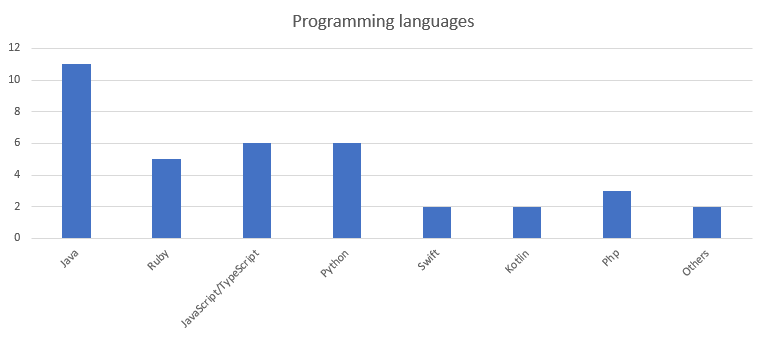
\includegraphics[width=\textwidth]{figures/interview/Question3.png}
\caption{Answers to Question 3 of the interview}
\label{fig:interview-3}
\end{center}
\end{figure}

\subsubsection{Dependency Management}

The 15 interviewees have experience with dependency management. However, some of them indicated that it is not a task that they usually perform in their jobs, but rather in personal projects or from time to time. Figure \ref{fig:interview-6} shows the answers to question 6, regarding the importance of updating the dependencies. The reasons given by the interviewees answering \textit{Neutral} and \textit{Important} for not giving it more importance include: prioritizing the fact that the versions used are compatible, that there are no version incompatibilities with the current version used, and that the version used is stable.

\begin{figure}[ht]
\begin{center}
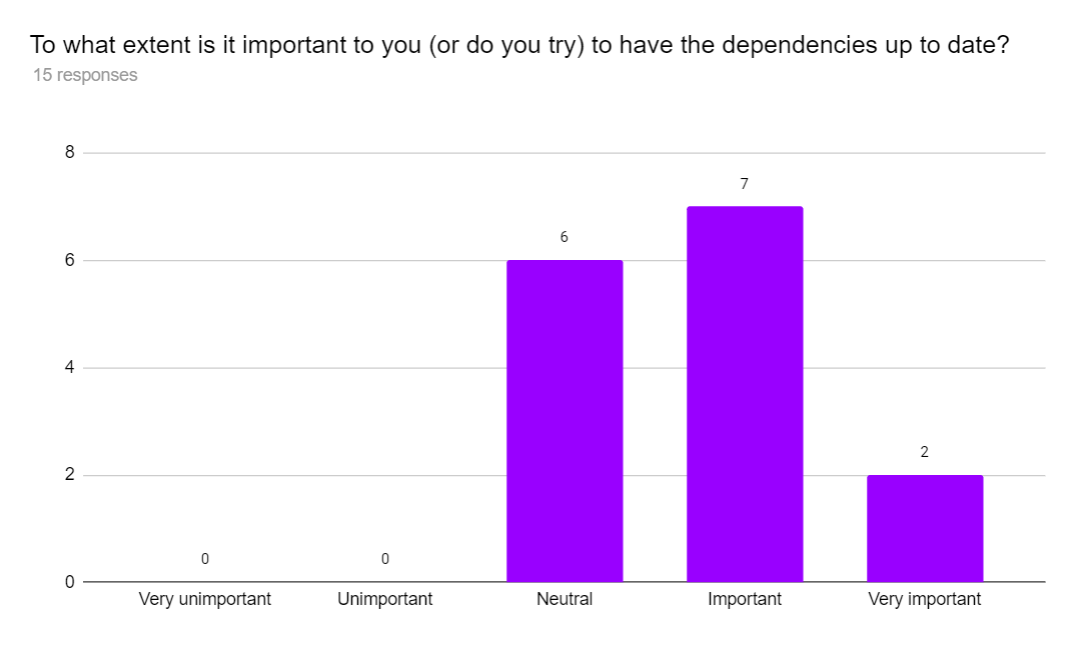
\includegraphics[width=\textwidth]{figures/interview/Question6.png}
\caption{Answers to Question 6 of the interview}
\label{fig:interview-6}
\end{center}
\end{figure}

 Figure \ref{fig:interview-7} the answers to question 7, about the importance of monitoring the vulnerabilities of the dependencies. The interviewees considering that the importance of monitoring the vulnerabilities of the dependencies was less than \textit{Very important} reasoned about it. For example, some said that it is something that they do, but not regularly. Also, they just update when there is a new version, to make sure that if a vulnerability has been discovered, the patch is always used. Finally, the last reason is that depends on the type of dependency that it is, since if it is not a customer-facing dependency, it is not that important.

\begin{figure}[ht]
\begin{center}
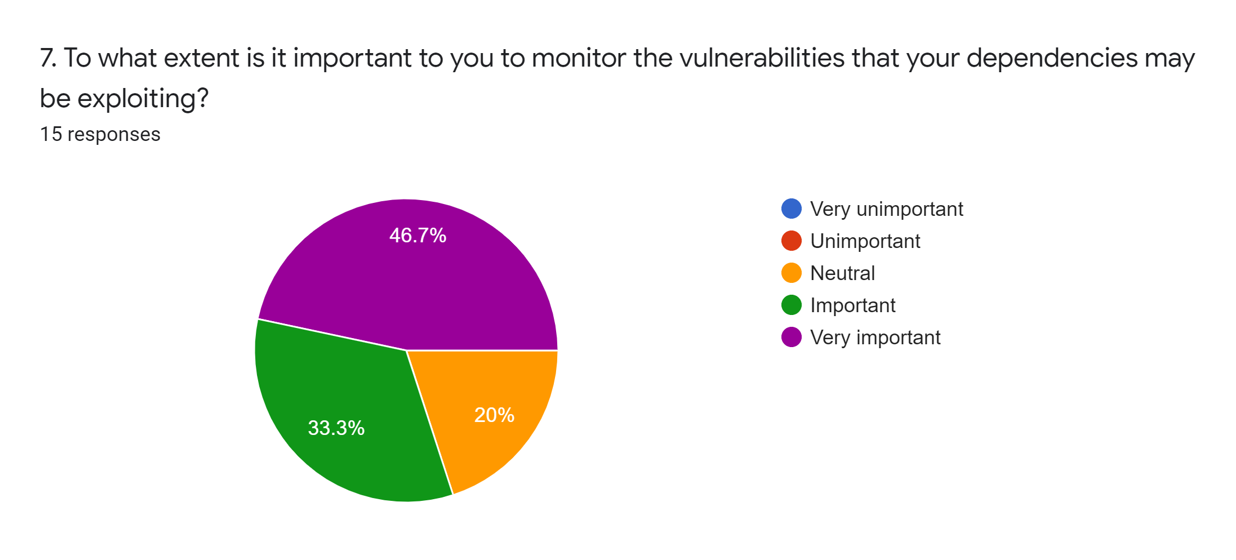
\includegraphics[width=\textwidth]{figures/interview/Question7.png}
\caption{Answers to Question 7 of the interview}
\label{fig:interview-7}
\end{center}
\end{figure}

In Figure \ref{fig:interview-8}, there are the answers to question 8. The interviewees gave more than one answer to the question, but always at least one explicitly included in the figure.

\begin{figure}[ht]
\begin{center}
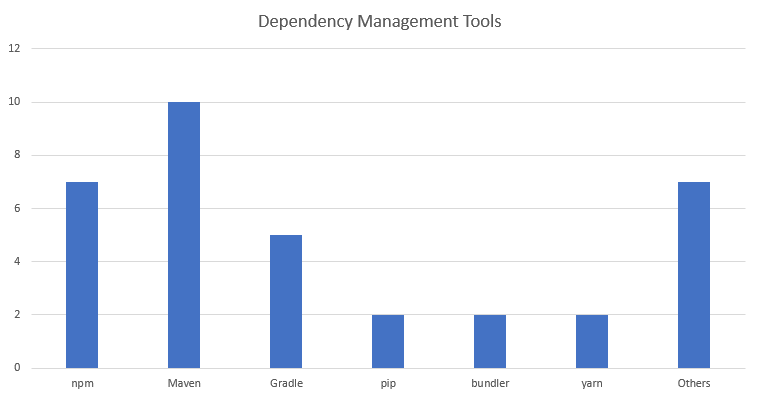
\includegraphics[width=\textwidth]{figures/interview/Question8.png}
\caption{Answers to Question 8 of the interview}
\label{fig:interview-8}
\end{center}
\end{figure}

Finally, the answers to question 9, regarding the how helpul are the tools that the interviewees use for dependency management are. The interviewees that considered the tools to be really helpful (5), compared it to not using any tool at all. Whilts the interviewees giving lower marks (2-3), considered that there are features missing. Mainly, they considered that the basic needs are covered, however some more detailed information about how to manage the dependencies is not there.

\begin{figure}[ht]
\begin{center}
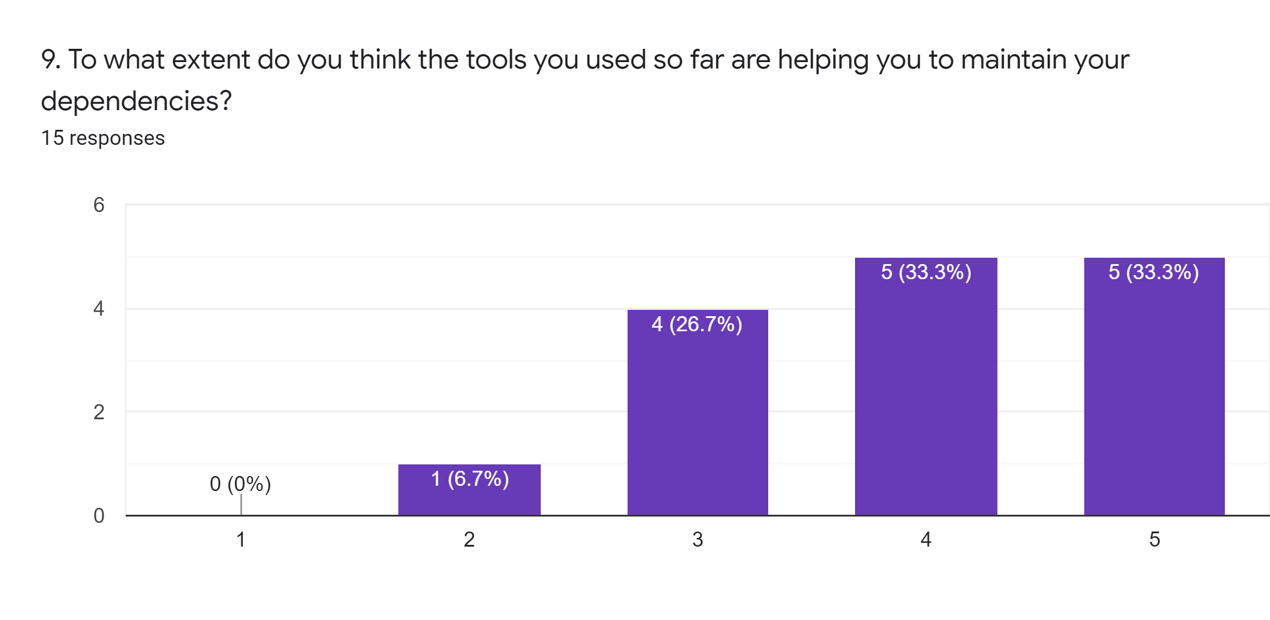
\includegraphics[width=\textwidth]{figures/interview/Question9.png}
\caption{Answers to Question 9 of the interview}
\label{fig:interview-9}
\end{center}
\end{figure}

\subsubsection{Visualizations}

The answers of the interviewees to question 10, about the usefulness of the tool are displayed in Figure \ref{fig:interview-10}. Some of the reasons of the interviewees for not giving it the maximum grade, are the need for improvement in some aspects of both the visualization and the metrics, as well as being useful for some very specific scenarios.

\begin{figure}[ht]
\begin{center}
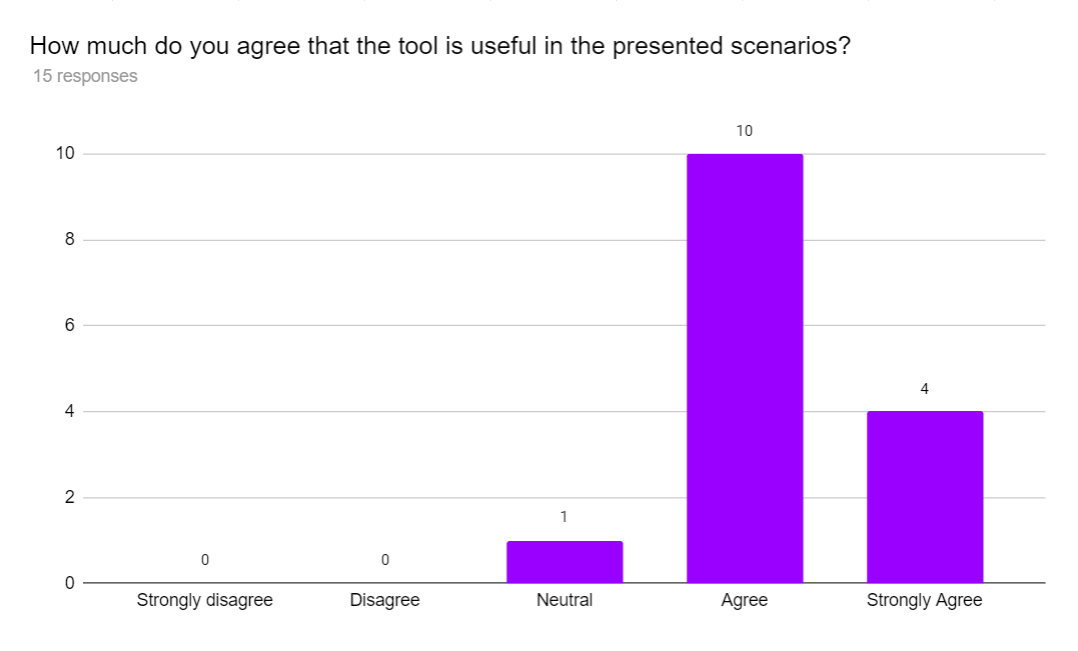
\includegraphics[width=\textwidth]{figures/interview/Question10.png}
\caption{Answers to Question 10 of the interview}
\label{fig:interview-10}
\end{center}
\end{figure}

Figure \ref{fig:interview-11} we can see the results for Question 11. In this case, the interviewees who answered \textit{Disagree} or \textit{Neutral} considered that the tool is meant for some very specific cases, which are not very likely to be needed. The other interviewees agreed that the tool would probably not be used on a daily basis, but would make some tasks easier, such as the ones discussed in the scenarios.

\begin{figure}[ht]
\begin{center}
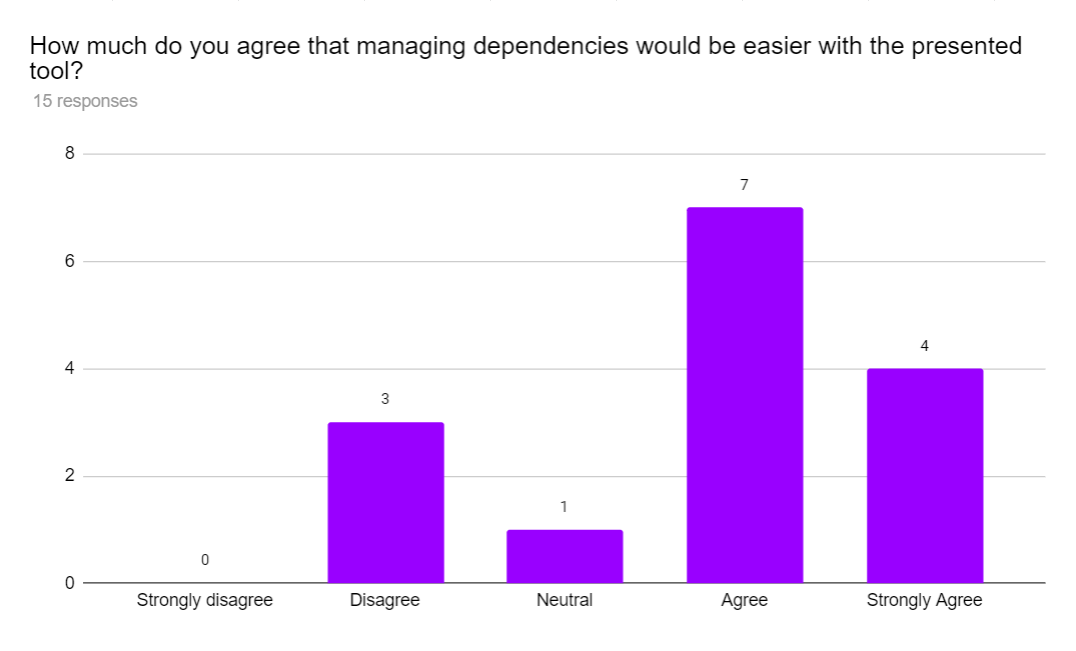
\includegraphics[width=\textwidth]{figures/interview/Question11.png}
\caption{Answers to Question 11 of the interview}
\label{fig:interview-11}
\end{center}
\end{figure}

For Question 12, about which of the visualizations are most useful, most of the interviews answered with more than one visualization. Table \ref{table:interview-12} summarizes the answers. The $\oplus$ indicates that the interviewee considered that visualization to be the most useful, and the $\odot$ is used when the interviewee said that the visualization was useful but in a clear second position. If the cell is empty, the interviewee did not mention the visualization in the answer.

\begin{table}[ht]
    \begin{center}
    \begin{tabular}{|c|c|c|}
    \hline
    Tree      & Table     & Barchart \\
    \hline\hline
    $\odot$   & $\oplus$  & ~        \\\hline
    ~	        & ~	        & $\oplus$ \\\hline
    $\oplus$  & ~         & $\oplus$ \\\hline
    $\oplus$	& ~         & ~        \\\hline
    $\oplus$	& $\odot$	  & $\oplus$ \\\hline
    $\oplus$	& ~         & $\odot$  \\\hline
    $\odot$	  & $\oplus$	& ~        \\\hline
    $\oplus$	& $\oplus$	& $\oplus$ \\\hline
    ~	        & ~	        & $\oplus$ \\\hline
    $\odot$	  & $\odot$	  & $\oplus$ \\\hline
    $\oplus$	& $\oplus$	& $\oplus$ \\\hline
    $\oplus$	& ~	        & ~        \\\hline
    $\oplus$	& $\oplus$	& $\oplus$ \\\hline
    $\odot$	  & ~	        & $\oplus$ \\\hline
    $\oplus$	& $\oplus$	& $\oplus$ \\\hline
    \end{tabular}
    \end{center}
    \caption{Answers to Question 12 of the interview}
    \label{table:interview-12}
\end{table}

The answers to Question 13, are shown in Figure \ref{fig:interview-13}. Just as in Question 11, the reason given by the interviewees who answered \textit{Disagree} or \textit{Neutral} are that the tasks for which the tool is useful are not one of the regular tasks in their job.

\begin{figure}[ht]
\begin{center}
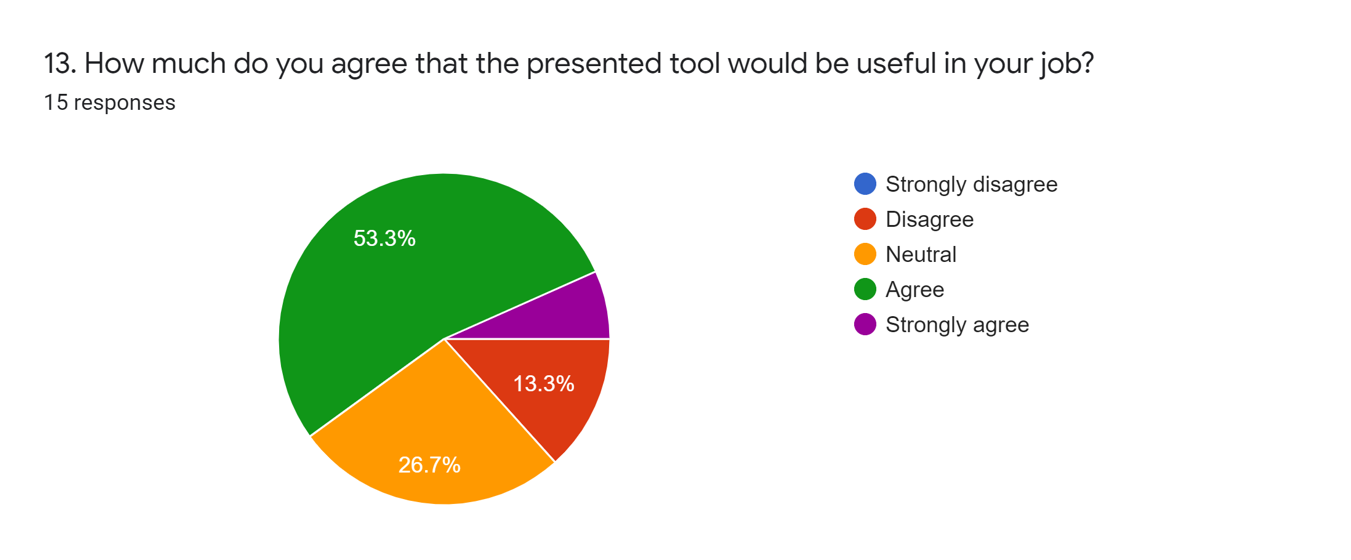
\includegraphics[width=\textwidth]{figures/interview/Question13.png}
\caption{Answers to Question 13 of the interview}
\label{fig:interview-13}
\end{center}
\end{figure}

With Question 14, the interviewees gave their suggestions for improvements of the current visualizations, as well as completely new visualizations. The list of suggestions can be found below:

\begin{itemize}
  \item Add tree visualization at the class level.
  \item List with the classes and methods used from a library.
  \item Add a decision making model, indicating which actions should be taken.
  \item Visualization to know how much of my system is depending on a library.
  \item Smart visualization displaying some potential problems: freshness of the dependency, multiple versions of the same library being used.
  \item Color legend in the tree map.
  \item Tooltip with a description of the metrics of the model.
  \item Display the licenses of the dependencies.
  \item Change the barchart for a table.
  \item Possibility to move and reorganize the nodes of the tree.
  \item Turn the features into a command interface, so it can be unatendedly running in the build pipeline.
\end{itemize}

\subsubsection{Metrics}

The answers to question 15 can be found in Figure \ref{fig:interview-15}, for each metrics the amount of times that an interviewee answered with each number of the options. In addition, Table \ref{table:interview-15} shows the average grade given to each metric.

\begin{figure}[ht]
\begin{center}
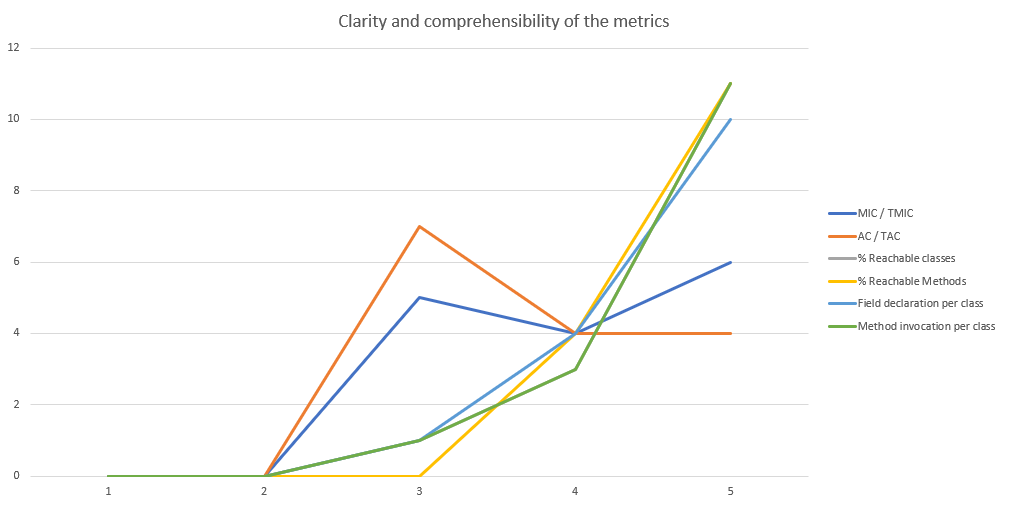
\includegraphics[width=\textwidth]{figures/interview/Question15.png}
\caption{Answers to Question 15 of the interview}
\label{fig:interview-15}
\end{center}
\end{figure}

\begin{table}[ht]
    \begin{center}
    \begin{tabular}{|l|l|}
    \hline
    Metric & Average \\
    \hline
    MIC/TMIC & 4.06 \\
    AC/TAC & 3.8 \\
    \% Reachable classes & 4.66 \\
    \% Reachable methods & 4.73 \\
    Field declaration per class & 4.6 \\
    Method invocation per class & 4.66 \\
    \hline
    \end{tabular}
    \end{center}
    \caption{Average grade of the metrics in Question 15}
    \label{table:interview-15}
\end{table}

In Figure \ref{fig:interview-16}, there are the answers to question 16 of the interview. The reasons for not giving the metrics the best grade include that it would be more useful if the metrics suggested as missing in question 19 were included. Also, it was suggested that context is missing for some metrics (e.g. the absolute number of reachable methods and classes, risk assessment for the coupling metrics).

\begin{figure}[ht]
\begin{center}
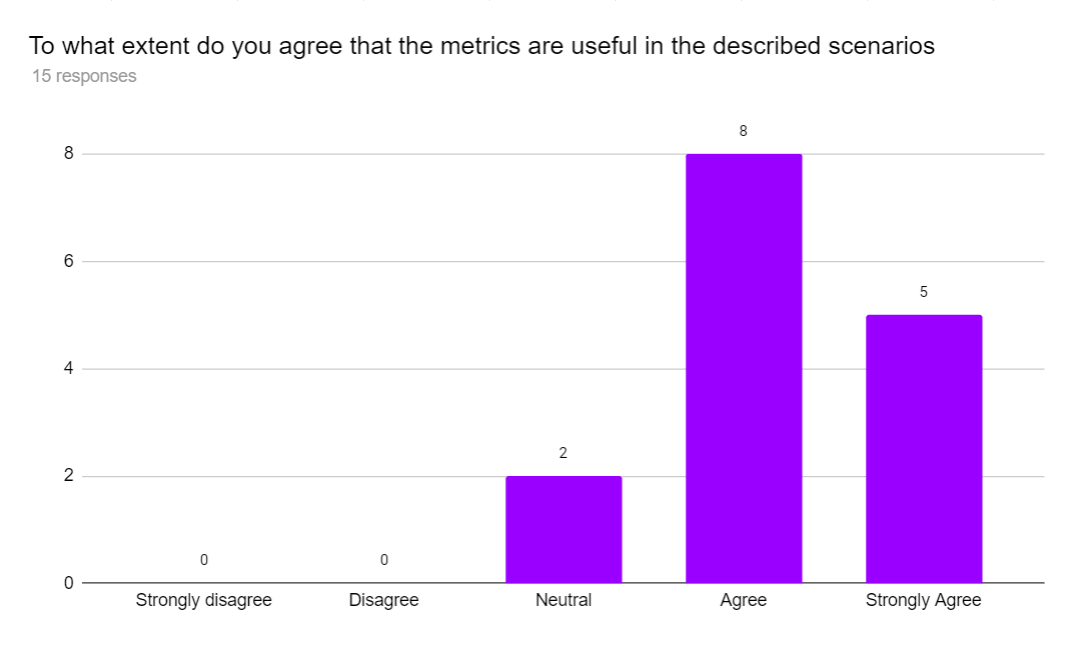
\includegraphics[width=\textwidth]{figures/interview/Question16.png}
\caption{Answers to Question 16 of the interview}
\label{fig:interview-16}
\end{center}
\end{figure}

The answers to question 17, can be found in Figure \ref{fig:interview-17}. The interviewees which gave a grade of \textit{Neutral}, reasoned that the metrics need some improvements to be really actionable, and that there is information that still can only be found in other places. The interviewees who answered \textit{Agree}, suggested that the metrics of the model are a good starting point, in order to know which actions to take, to start with.

\begin{figure}[ht]
\begin{center}
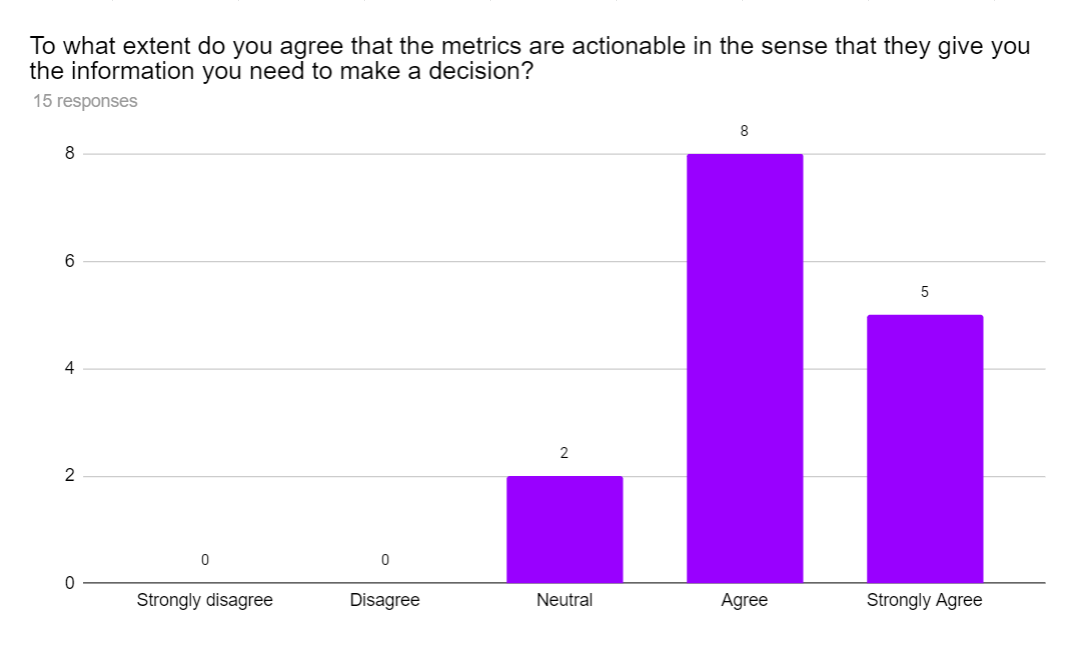
\includegraphics[width=\textwidth]{figures/interview/Question17.png}
\caption{Answers to Question 17 of the interview}
\label{fig:interview-17}
\end{center}
\end{figure}

For question 18, the interviewees answered with which metrics they considered more useful. Their answers can be found in Table \ref{table:interview-18}. As in question 12, an $\oplus$ means that the interviewee mentioned the metric as one of the most useful, $\odot$ is for the metrics mentioned in a second place. And finally, if the cell is empty means that the metric was not mentioned.

\begin{table}[ht]
    \begin{center}
    \begin{tabular}{|c|c|c|c|c|c|}
    \hline
    \rot{MIC / TMIC}	& \rot{AC / TAC}	& \rot{\% Reachable classes}	& \rot{\% Reachable Methods}	& \rot{Field declaration per class}	& \rot{Method invocation per class    } \\
    \hline\hline
    $\oplus$  & ~	       & $\oplus$	& ~	        & ~	        & ~        \\\hline
    ~	        & ~	       & $\oplus$	& $\oplus$	& ~	        & ~        \\\hline
    ~	        & ~	       & $\oplus$	& $\oplus$  & ~	        & ~        \\\hline
    ~	        & ~	       & ~	      & ~	        & $\odot$	  & $\oplus$ \\\hline
    ~	        & ~	       & $\oplus$	& $\oplus$	& ~	        & ~        \\\hline
    ~	        & ~	       & $\oplus$	& $\oplus$	& ~	        & ~        \\\hline
    $\oplus$	& ~	       & $\oplus$	& $\oplus$	& ~	        & ~        \\\hline
    $\oplus$	& ~	       & ~	      & ~	        & ~	        & ~        \\\hline
    $\oplus$	& $\oplus$ & $\oplus$	& $\oplus$	& ~	        & ~        \\\hline
    ~	        & ~	       & $\oplus$	& $\oplus$	& $\oplus$	& $\oplus$ \\\hline
    $\oplus$	& $\oplus$ & $\oplus$	& $\oplus$	& $\oplus$  & $\oplus$ \\\hline
    $\oplus$	& $\oplus$ & ~	      & ~	        & ~	        & ~        \\\hline
    $\oplus$	& $\oplus$ & ~	      & ~	        & ~	        & ~        \\\hline
    ~	        & ~        & $\oplus$ & $\oplus$	& ~         & ~        \\\hline
    $\oplus$	& ~	       & $\oplus$ & ~	        & ~	        & ~        \\\hline
    \end{tabular}
    \end{center}
    \caption{Answers to Question 18 of the interview}
    \label{table:interview-18}
\end{table}

Finally, the suggestions made for improving the current metrics or adding new ones, in the answers of question 19, can be found in the list below:

\begin{itemize}
  \item Min, max, and mean of the coupling metrics.
  \item How much of the client is depending on the server library.
  \item A list of the reachable methods and classes.
  \item The absolute number of reachable methods and classes.
  \item Freshness indicator.
  \item Aggregate of the coupling metrics.
  \item Muber of files of the client using the server library.
  \item Lines of code of the client affected by the dependency.
  \item Code reuse: a combination of the metrics.
\end{itemize}

\section{Experiment 5: Benchmarking}
One of the main remarks received for the coupling metrics during the interviews, is that there is not a clear scale for those metrics. Therefore, the value of the metrics can be hard to interpret, since there is no indicator of which number is very high or very low.

Hence, we have done a benchmarking of the values of the metrics \texttt{MIC}, \texttt{AC}, \texttt{TMIC}, and \texttt{TAC}. The goal is to understand which is the distribution of the values, and be able to indicate which are the outliers of these metrics.

\subsection{Experimental set up}
To execute this experiment, we have set a new request in the backend of the PoC. This request should contain the path to a \textit{.txt} file which includes three different columns, tab delimited. Each row represents a Maven artifact, and for each column it indicates: \textit{group id}, \textit{artifact id}, and \textit{version}.

Then, the calculation of the metrics of the model is performed. For each analyzed dependency, the value of the benchmarked metrics is stored. The result consists on 4 different \textit{.csv} files. The first two, containing all the different values of the \texttt{MIC} and \texttt{AC} metrics respectively. The last files represent the values of the transitive coupling metrics, represented in three columns. The first, the dependency id, the second the distance, and the third the value calculated at the distance. Therefore, more than one row might be used to represent the \texttt{TMIC} or \texttt{TAC} of a dependency.

\subsection{Results}
